% This is samplepaper.tex, a sample chapter demonstrating the
% LLNCS macro package for Springer Computer Science proceedings;
% Version 2.21 of 2022/01/12
%
\documentclass{llncs}
%
\usepackage[T1]{fontenc}
% T1 fonts will be used to generate the final print and online PDFs,
% so please use T1 fonts in your manuscript whenever possible.
% Other font encondings may result in incorrect characters.
%
\usepackage{graphicx}
\usepackage{cite}        
% Used for displaying a sample figure. If possible, figure files should
% be included in EPS format.
%
% If you use the hyperref package, please uncomment the following two lines
% to display URLs in blue roman font according to Springer's eBook style:

\documentclass{article}

\usepackage{subfigure} % Or \usepackage{subcaption} for subfigures
\usepackage{float}     % For using [H]
%\usepackage{color}
%\renewcommand\UrlFont{\color{blue}\rmfamily}
%
\begin{document}
%
\title{Enhancing Cloud Security with Deep Learning - An ANN
Approach for Cyber Threat Detection}
%
%\titlerunning{Abbreviated paper title}
% If the paper title is too long for the running head, you can set
% an abbreviated paper title here
%
\author{M.Sathyam Reddy\inst{1} \and
Gattu Thanuja\inst{2} \and
Rama Krishna Eluri\inst{3} \and
Bojja Sobharani\inst{4} \and
Thalapaneni Suma Durga\inst{5} \and
Dodda Venkata Reddy\inst{6} \and
Moturi Sireesha\inst{7}
}

\authorrunning{M.Sathyam Reddy}
\titlerunning{Cloud Security with ANN for Threat Detection}

\institute{
 \inst{1,2,3,4,5,6,7}Department of CSE, Narasaraopeta Engineering College, Narasaraopeta, Palnadu district, Andhra Pradesh, India \\
 \email{sathyamreddym@gmail.com}
}
%
\maketitle             % typeset the header of the contribution
%
\begin{abstract}
Due to the increasing role of cloud computing in the growth of trustable digital services, secure and efficient solutions will be a must in the mitigation of cyber risks. This paper presents an approach to the enhancement of cloud security through the application of deep learning, focusing on Artificial Neural Networks. Moderate segments of ANN algorithms have been performed that are Levenberg-Marquardt(LM), Scaled Conjugate Gradient(SCG) and Bayesian Regularization(BR), to build an enhanced threat detection system which has the capability of detecting highly complex attacking patterns in the cloud.The paper also looks at the problem of various types of cyber threat detection - malware, phishing, distributed denial of service (DDos) attacks etc. Finally, it can be concluded that employing the knowledge of ANN, and other, deep learning approaches, can facilitate the development of persistent cyber defense structures in the cloud. The research shows how ANN models can contribute to a faster and easier detection of new, unclassified threats, therefore increasing the overall security of cloud related activities.

\keywords{Cloud computing, cyber threat detection, Deep Learning,
Levenberg-Marquardt algorithm, scale conjugate gradient, Bayesian Regu
-larization, Artificial Neural Networks (ANNs).}
\end{abstract}
%
%
%
\section{Introduction}
The emergence of cloud computing has fundamentally altered how people and organizations store, manage, and access information. It provides previously unheard of scale and flexibility [1]. Because cloud systems are centralized, they are attractive targets for cybercriminals, who are always coming up with more complex and varied ways to take advantage of weaknesses [15]. As a result, new adaptive and intelligent security responses that can detect and neutralize threats in real time are not readily available. Ability to improve cloud system cyber security.In particular, artificial neural networks (ANNs) have shown remarkable ability to detect and identify complex patterns in large data sets [2].They are particularly adept at both known and unknown threats because of their ability to adapt and learn from past attacks[2]. This paper investigates the application of deep mastering strategies, which specialize in ANNs [2], to enhance cloud safety through superior cyber threat detection.
\subsection{Contribution of the wrok}
Construct a ANN model for detecting the cyber threats. \\
• Initially ANN is used to train the version with a dataset (CICIDS 2017 data set and UNSW-NB15 data set). \\
• Using the other dataset that can be the Malicious URLs Dataset.\\
• Experiment and compare the performance through the acquired outcomes. \\
An Artificial Neural Network version is created to detect cyber threats and other facts of the community. Initially, the ANN model is trained with CICIDS 2017, UNSW-NB15 datasets, and testing can be done with the same datasets. Finally, the performance is compared with the other models and one can easily detect cyber threats. 



\section{Literature Review}
In addition to providing flexibility, scalability, and performance comparable to standard not exceptional performance, cloud computing also adds security risks such as virus attacks, insider threats, and data breaches[3]. Unauthorised access to sensitive cloud records is one kind of a data breach that can cause harm to one’s finances and reputation. Insider threats
originate from criminal clients who abuse their access to steal data or interfere with business operations. Traditional protection capabilities, such as firewalls and antivirus software, are regularly inadequate to cope with evolving threats, as they will be inclined to react and might not discover superior or zero-day attacks in real time [3]. Deep mastering,
a subset of model study, shows great capability in improving cybersecurity. Models like Artificial Neural Networks (ANNs)[2] can pick out complex styles in massive datasets, making them suitable for detecting anomalies and predicting functionality threats.


\section{Data Collection}
Various datasets related to cyber threats are available on Kaggle.com, and data can be sourced from these datasets. One known dataset is CICIDS 2017[4], which contains a variety of the community attack scenarios and covers the wide range of cyber threats induced by DDos, web-based and botnet attacks among others.This dataset also contains the real-world data. This dataset is useful in studying the trends and characteristics of different cyber attacks helping in the determination of the weak points of cloud scenarios and coming up with effective counter measures. Another dataset is UNSW-NB15[4], which consists of arranged files providing useful information to separate normal and harmful traffic patterns.
Other dataset is Malicious URLs dataset, which consists of malicious data 
like Links.To summarise, these datasets are helping in getting a holistic view of the dialogue of the problem, which enhances incoming changes in industry practices in challenge anticipation and resilience development thus better cyber safety.
\section{PREPROCESSING}
Preprocessing comes down to two major parts, namely: scaling of the features and encoding of the features. The aim of feature scaling is to put all the numeric values in some appropriate range, for instance, by using Min-Max scaling or Z-score normalization in order to avoid situations where features with bigger values are the ones that are in control of the model’s learning process [5]. Label encoding is basically converting the categorical features into numerical form by filling ordinal categories with label encoding and non-ordinal with one-hot encoding [12]. All these steps helps to improving their models performance and efficiency by making sure that the information is well organized. Without proper preprocessing, it would be rather impossible, for instance, to achieve the efficiency of the models as they will be unable to understand the structures of the different datasets.
\subsection{Feature Scaling}
Apply feature scaling in order to guarantee that all the different parameters associated with the network (such as the number of bytes, the duration of active sessions, the rates of packets, and so on) are at a similar range. 
\subsection{Label Encoding}
It is necessary to encode the labels. Attack labels should be converted to numbers, which is where label encoding comes in. This is not difficult if one is doing an attack detection with only benign classes such as attack and benign. However, in cases where there are several classes of attacks, encoding technique employs one hot encoding or embeddings.
\section{PROPOSED ANN MODEL}
The cloud security approach which relies on using an Artificial Neural Network (ANN) as proposed in this work starts with the appropriate selection and processing of data from both the CICIDS 2017,the UNSW-NB15 dataset and the Malicious URLs dataset. Due to the massive scale of the datasets, 10 percent sample of the preprocessed data is utilized for expediency. The partitioning is performed such that 70 percent  of the data is used for training while the rest 30 percent is used in testing and validating the model building to ensure model generalization and performance checking. The architecture of ANN involves an commonly layered input layer containing the features of the dataset, four hidden layers which uses ReLU transformation to model non-linear relationships, and the output layer which depends on the nature of the task whether to be one of several classes or binary. The model is trained with the following three algorithms, Levenberg-Marquardt, Scaled Conjugate Gradient and Bayesian Regularization . The number of hidden layers, learning rates, batch sizes, and similar factors are regulated after tuning, dropout and other similar techniques are used for generalization. In evaluating the performance of the model, its major purposes have been accuracy, precision, recall, F1 scores, any measure that can help in reduction of false positives and false negatives.
As soon as the ANN model is validated it can be deployed in a cloud environment offering real time cyber threat detection by making use of cloud computing architecture for real time network traffic analysis.

The Levenberg-Marquardt (LM) algorithm helps attain faster convergence on smaller datasets with difficult models, effectively describing non-linear patterns of network traffic for improved accuracy in detection. The Scaled Conjugate Gradient (SCG) algorithm is appropriate for many data sets, more so cloud environments due to its superior methods of memory usage and stability in training allowing the model to learn efficiently from high dimensional data. At the same time, the probabilistic approach called Bayesian Regularization (BR) is essential to control the overfitting of the neural network, as it helps the ANN to be applicable with new types of attacks not seen during the ANN training and provides estimates of the uncertainty of the prediction which assists in making important security decisioning response to threats. From the integration of these algorithms, efficient and fast training and performance in fighting cyber threats can be realized in your project.


\subsection{Feed-forward Neural Network:}
A feed-forward neural network with L layers can be represented as a series of matrix multiplications and activation functions.For each layer $l$ from $1$ to $L$:

\begin{equation}
c^{[l]} = g^{[l]}(W^{[l]} \cdot c^{[l-1]} + d^{[l]})
\end{equation}

where:
\begin{itemize}
    \item $c^{[l]}$ is the activation of layer $l$,
    \item $W^{[l]}$ and $d^{[l]}$ are the weight matrix and bias vector for layer $l$,
    \item $g^{[l]}$ is the activation function (e.g., ReLU, sigmoid).
\end{itemize}
\begin{table}[htbp]
\caption{Comparing the ANN model with other models}
\centering
\begin{tabular}{|c|c|c|}
        \hline
        SNo & Model & Accuracy \\ \hline
        1 & ANN & 90.20 \\ \hline
        2 & CNN & 86.58 \\ \hline
         3& RNN & 87.84 \\ \hline
        4 & LSTM & 79.00 \\ \hline
        5 & AutoEncoders & 86.01 \\ \hline
        6 & SVM (Original) & 84.74 \\ \hline
        7 & SVM (Encoded) & 84.95 \\ \hline
\end{tabular}
\label{tab 1}
\end{table}
The table-1 illustrates how well different models are able to detect cyber threats based on deep learning model performances, with the graphical representation of performance showing that the ANN model is the preferable choice. The ANN scores the peak accuracy of 90.20 and it is thus scored as the most accurate model in this case. As opposed to that video analytics, the convolutional neural network sets the next record with accuracy 86.58. While the Recurrent neural network shows close results at 87.84. Touching on the LSTM responsible for attaining the lowest accuracy level at 79.00 and going further to the AEs with 86.01. The plain letric Support Vector Machine benchmarking an accuracy of 84.74, the encoded SVM resolving the performance deviate of 84.95. On the spine though ANN has the least chance of being the preferred model in cyber threat detection, it has outperformed all the other deep learning models.

\begin{figure}[htbp]
    \centering
    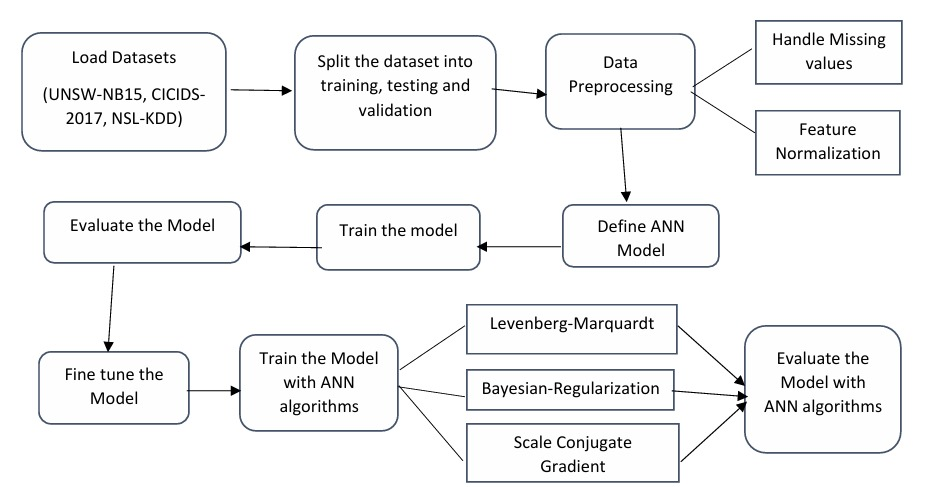
\includegraphics[width=1\linewidth]{image.png}
    \caption{Proposed Artificial Neural Networks Model Architecture}
    \label{fig:enter-label}
\end{figure}
The figure-1 presents a framework for the detection of cyber threats based on the use of Artificial Neural Networks (ANN) and two datasets, namely, CICIDS-2017 and UNSW-NB15. The first stage of the methodology is concerned with importing such datasets which consist of both clean and a testing dummy data and then dividing the information into training, testing, and validation samples in order to improve the model. Then, a data-ready solution is created by eliminating rows with missing values as well as standardizing all characteristics of the data set. A neural network model is built, where configuration settings including inputs, hidden layers and outputs are created in consideration of the objective which is cyber threat detection. Beginning with the Levenberg-Marquardt algorithm that guarantees that convergence will be speeded up, then Bayesian Regularization which is included to mitigate the overfitting of the ANN and lastly, Scaled Conjugate Gradient which is used for solving large datasets. Also, the model’s performance is assessed using various metrics such as accuracy, precision, recall, and F1 score to demonstrate that the model is able to identify cyber threats. If necessary, hyperparameter tuning is added to the model in order for the latter one to be the best possible. Enhanced threat detection centered on the CICIDS-2017 and UNSW-NB15 datasets is the basis upon which the development of this approach rests.
\section{Performance Evaluation}
Performance evaluation proves to be vital when developing models especially for the purpose of detecting cyber security threats, because it determines the extent to which the model is effective in predicting outcomes when a different data not used during training is put into use [6]. For this reason, key metrics for evaluation include accuracy, which measures the ratio of predictions made accurately, precision which measures true positives normalized to positive predictions, certain threats detected are properly and also, recall defines how well the model can recognize numerous positive threats and the overall influences of preference over both precision and falseness, the F1-score, particularly noteworthy in class skewed data. This includes positive prediction, and negative prediction, as well as negative false accounts of a positive prediction, and vice versa, performance that pictorially explains the performance of the system [8]. Depending on these evaluations, the hyperparameters could be adjusted to improve performance and there is a need to keep tracking the relevant cyber defense mechanisms as threats are becoming more advanced.

The following graphs and tables are the performance metrics used in  ANN model.

\begin{figure}[htbp]
\hspace{-1.2cm}
    \subfigure{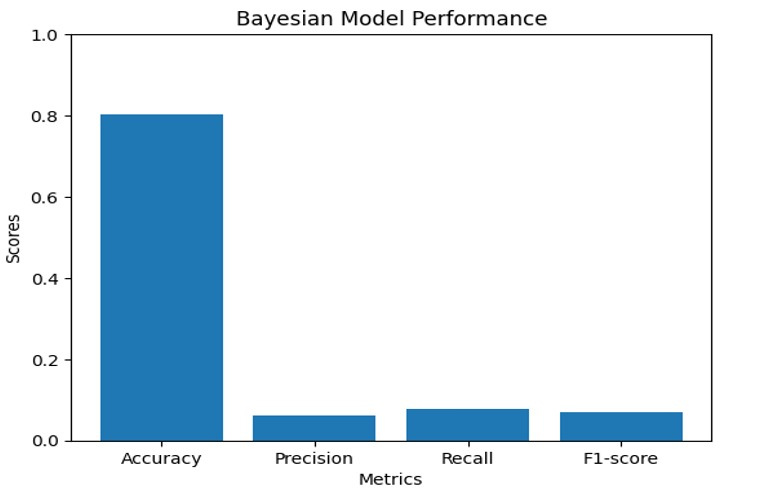
\includegraphics[width=0.59\textwidth]{1.png}}
    \hspace{-0.5cm}
    \subfigure{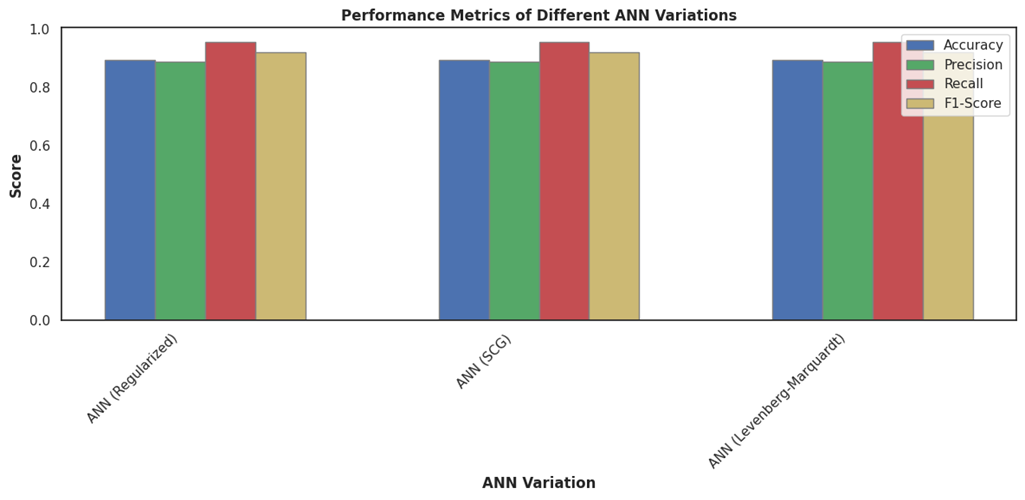
\includegraphics[width=0.59\textwidth]{2.png}}
    \caption{\small{Performance metrics for ANN Model}}
    \label{fig:abc}
\end{figure}

The figure-2 above represents the metrics used in the ANN model.
The coordinates of the adequate metrics of the Bayesian model are shown in the diagram. In this case, the x-axis displays the metrics, which include accuracy, precision, recall, and F1 score, while the y-axis encompasses the corresponding scores of the metrics. The model performed best on accuracy, precision came next, then recall, and finally the F1 score. It can be inferred from the above findings that the model makes correct predictions most of the time and manages to pinpoint almost all positive instances with very few false positives and false negatives [10]. No specific values were given though it can be assumed though that the model is performing at least on a satisfactory level with respect to the set metrics, especially the accuracy.\\

\subsection{Binary Conversion}

The model output is a probability value, which is converted to a binary prediction based on a threshold of 0.5. It is defined as:

\begin{equation}
y_{\text{pred\_binary}} =
\begin{cases}
1 & \text{if } y_{\text{pred}} > 0.5 \\
0 & \text{otherwise}
\end{cases}
\end{equation}

where \( y_{\text{pred}} \) is the predicted probability.

\begin{table}[htbp]
\caption{Dataset Information(UNSW-NB15)}
\centering
\begin{tabular}{|c|c|c|}
        \hline
        SNo & Data & Total Records \\ \hline
        1 & Training data & 18036 (70Percent) \\ \hline
        2 & Testing data & 3866 (15Percent) \\ \hline
        3& Validation data & 3865 (15Percent) \\ \hline
        4 & Total records & 25767 (100Percent)\\ \hline
\end{tabular}
\label{tab 2}
\end{table}

The table-2 explains the details of UNSW-NB15 Data set that has been utilized for assessing the performance of different ML models. There is a total of 25,767 records in the dataset, which are further separated into training, testing and validation datasets. Out of the total records of 18,036 records (70 percent), the training set contains 18,036 records, the test room has 3,866 records (15 percent), and the resale market has 3,865 records (15 percent). This distribution is good for modeling purposes such as training, testing, and validating models.
The UNSW and CICIDS are both used for implementing and for validation. We can compare with the other models ANN gives best results than other models. ANN model contains the training parameters of 13,253 and total number of optimizer params is 8,836 is shown in table-3 [11]. This comparison highlights the ANN’s superior effectiveness in this particular task, while also underscoring the varying performance of different models based on their parameter configurations[6].

% \begin{figure}[htbp]
%     \subfigure{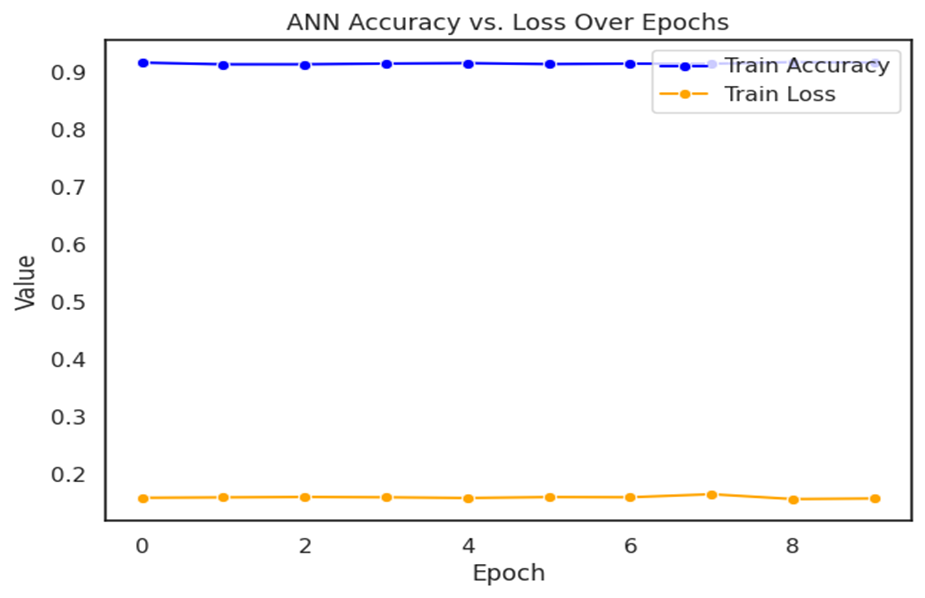
\includegraphics[width=0.59\textwidth]{3.png}}
%     \subfigure{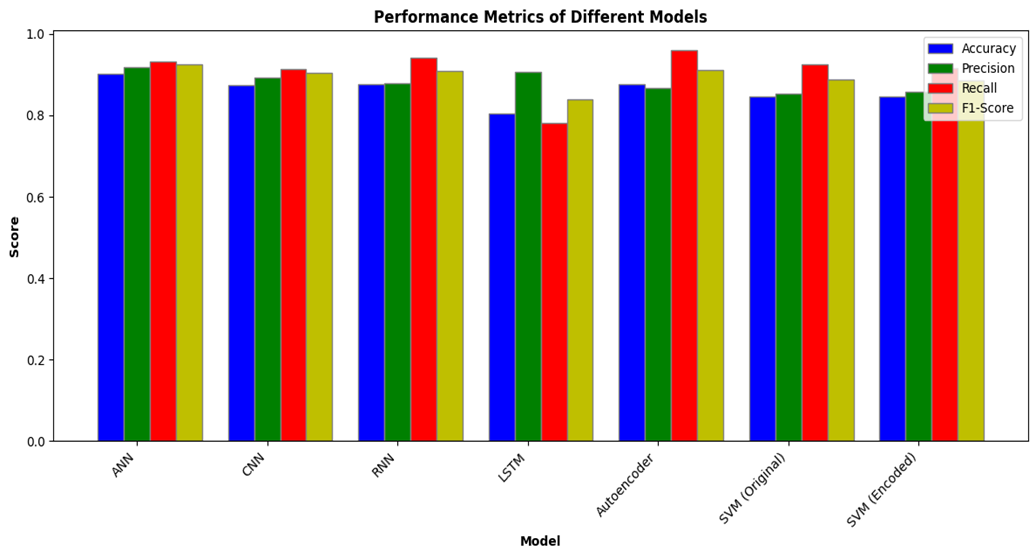
\includegraphics[width=0.59\textwidth]{4.png}}
%     \caption{\small{Performance metrics for ANN Model}}
%     \label{fig:abc}
% \end{figure}

% \begin{table}[htbp]
% \caption{Information about the models in UNSW-NB15}
% \centering
% \begin{tabular}{|c|c|c|c|c|}
%         \hline
%         Model & ANN & CNN & RNN & LSTM \\ \hline
%         Total Params & 13,253 & 99,269 & 19,013 & 57,029 \\ \hline
%         Trainable Params & 4,417 & 33,089 & 6,337 & 19,009 \\ \hline
%         Non-trainable params & 0 & 0 & 0 & 0 \\ \hline
%         Optimizer params & 8,836 & 66,180 & 12,676 & 38,020 \\ \hline
%         Accuracy & 90.12 & 87.30 & 87.69 & 80.44 \\ \hline
% \end{tabular}
% \label{tab 3}
% \end{table}


% \begin{figure}[htbp]
%     \centering
%     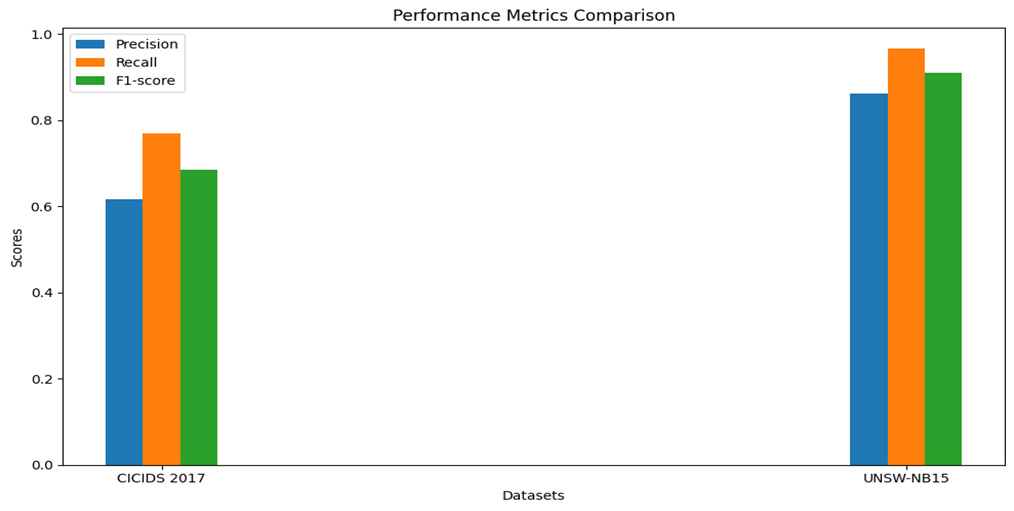
\includegraphics[width=0.75\linewidth]{5.png}
%     \caption{Comparsion of performance metrics for the both datasets UNSW and CICIDS}
%     \label{fig:enter-label}
% \end{figure}




\begin{figure}[H]
\hspace{-1.4cm}
    \subfigure{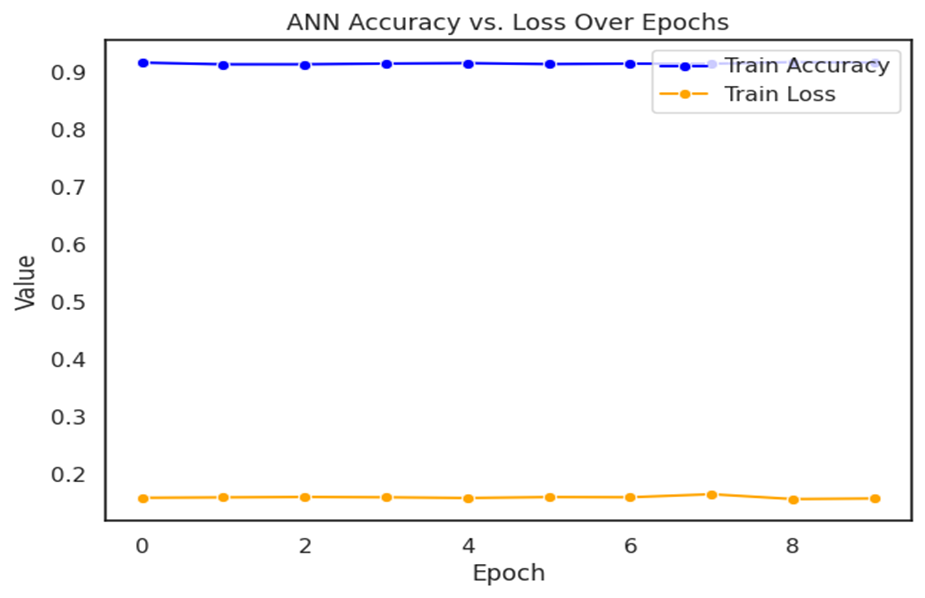
\includegraphics[width=0.59\textwidth]{3.png}}
    \subfigure{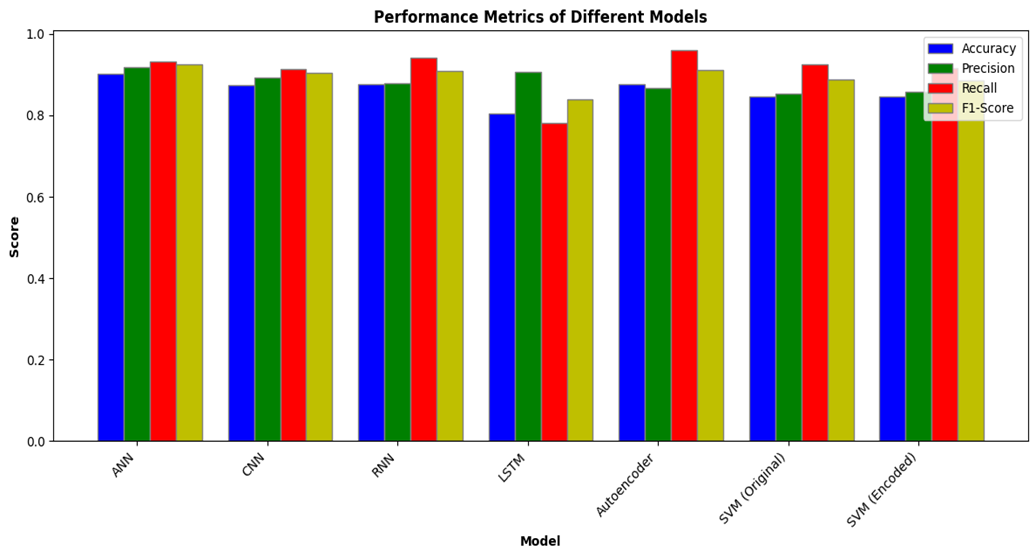
\includegraphics[width=0.59\textwidth]{4.png}}
    \caption{\small{Performance metrics for ANN Model}}
    \label{fig:abc}
\end{figure}
The figure-3 shows Line graph titled "ANN Accuracy vs. Loss Over Epochs" showing two lines: blue for train accuracy and orange for train loss. The x-axis represents epochs from 0 to 9, and the y-axis represents value from 0 to 1. The train accuracy remains consistently high around 0.9, while train loss stays low around 0.1 throughout the epochs.And also the Bar chart titled "Performance Metrics of Different Models" comparing accuracy, precision, recall, and F1-score across various models: ANN, CNN, RNN, LSTM, Autoencoder, SVM (Original), and SVM (Encoded). Each model is represented by four colored bars: blue for accuracy, green for precision, red for recall, and yellow for F1-score. Most models show high scores close to 1.0 across all metrics, with slight variations.

\begin{table}[H]
\caption{Information about the models in UNSW-NB15}
\centering
\begin{tabular}{|c|c|c|c|c|}
        \hline
        Model & ANN & CNN & RNN & LSTM \\ \hline
        Total Params & 13,253 & 99,269 & 19,013 & 57,029 \\ \hline
        Trainable Params & 4,417 & 33,089 & 6,337 & 19,009 \\ \hline
        Non-trainable params & 0 & 0 & 0 & 0 \\ \hline
        Optimizer params & 8,836 & 66,180 & 12,676 & 38,020 \\ \hline
        Accuracy & 90.12 & 87.30 & 87.69 & 80.44 \\ \hline
\end{tabular}
\label{tab 3}
\end{table}
\begin{figure}[H]
    \centering
    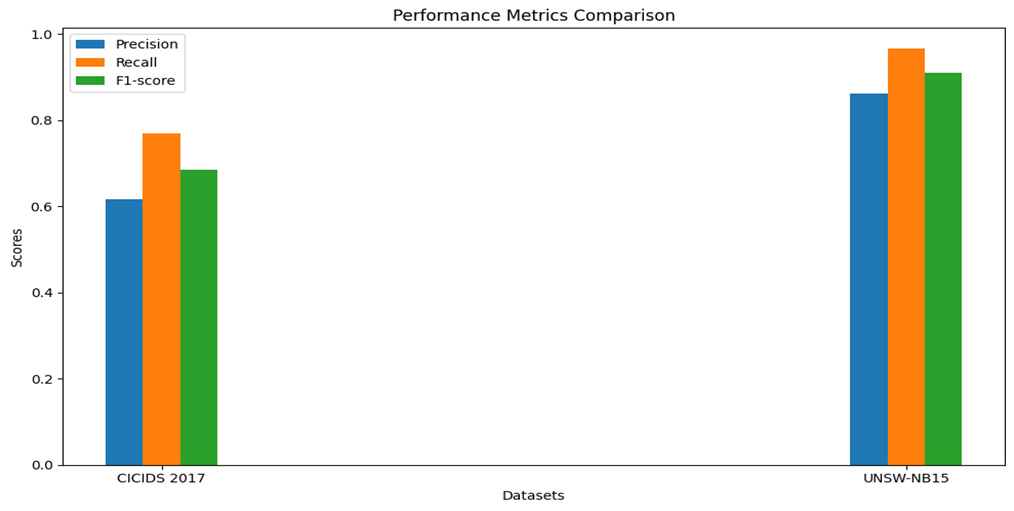
\includegraphics[width=0.75\linewidth]{5.png}
    \caption{Comparison of performance metrics for both datasets UNSW and CICIDS}
    \label{fig:enter-label}
\end{figure}




This analysis shows that each dataset produces a variation in the performance of the model, here, the ANN with emphasis on the characteristics of the datasets concerning their effects towards precision, recall, and F1-score.

\section{Comparative Analysis}
Over the last few decades, artificial neural networks (ANNs) have been recognized as one of the most effective possibilities for detecting cyber threats within the cloud security paradigm toolbox, achieving higher performance in the major metrics of accuracy, precision, recall, and F1 score in comparison with more basic models like SVM, CNN or RNN [7] in figure-5. ANNs excel in this situation as well since they are trained to recognize the non-linear patterns concealed in these large datasets such as UNSW-NB15 and CICIDS 2017 in figure-4, doing so with an edge in recall and F1 score, both of which are vital in lowering the rate of false negatives in such vital domains as cybersecurity. This trait allows it to be effectively operated in clouds, where mobile computing and the internet are dynamically changing. That gives ANNs the capability to work better in dynamic cloud environments where there is the potential of the threats changing [9]. This makes ANNs a main convincing reason to solve the problem of the cloud trust barriers by opening up the new security possibilities including but not limited to the detection of the unknown threats, which cannot be captured by the classical methods.
\begin{figure}[htbp]
\hspace{-0.8cm}
    \subfigure{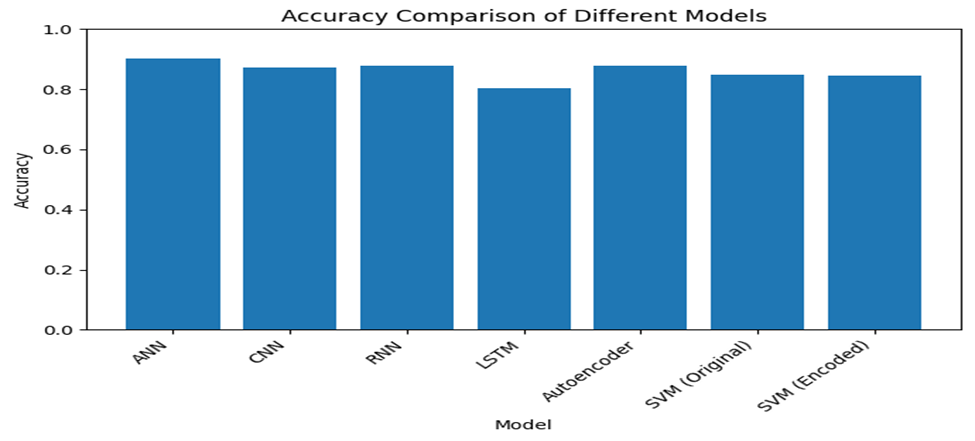
\includegraphics[width=0.59\textwidth]{6.png}}
    \subfigure{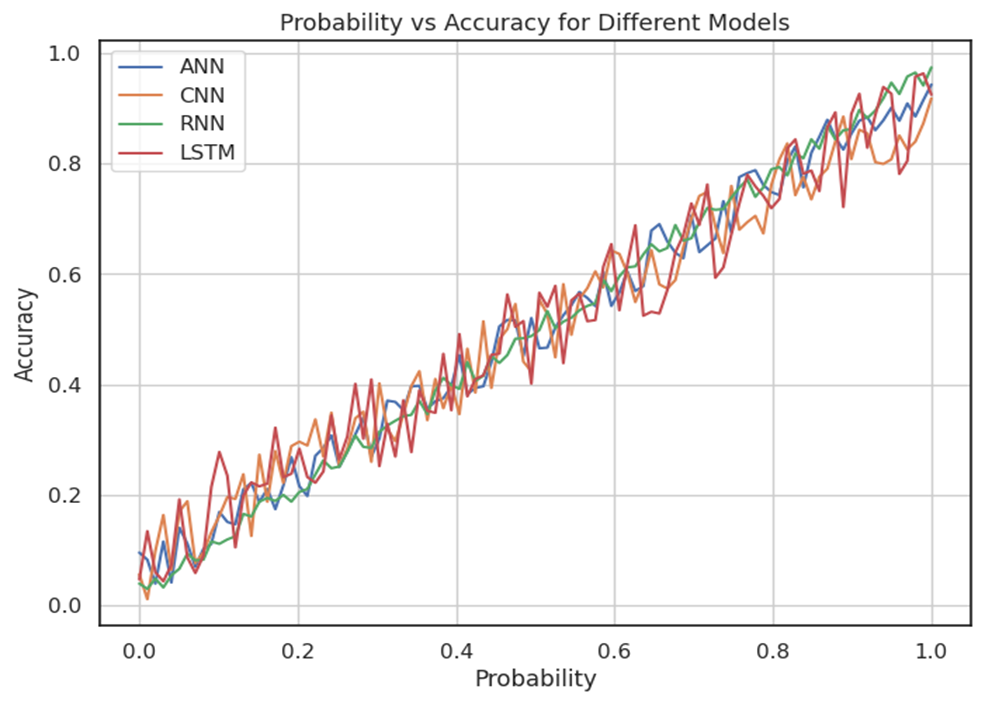
\includegraphics[width=0.49\textwidth]{7.png}}
    \caption{\small{Comparing ANN with the other models}}
    \label{fig:abc}
\end{figure}
\begin{figure}[htbp]
\hspace{-1.2cm}
    \subfigure{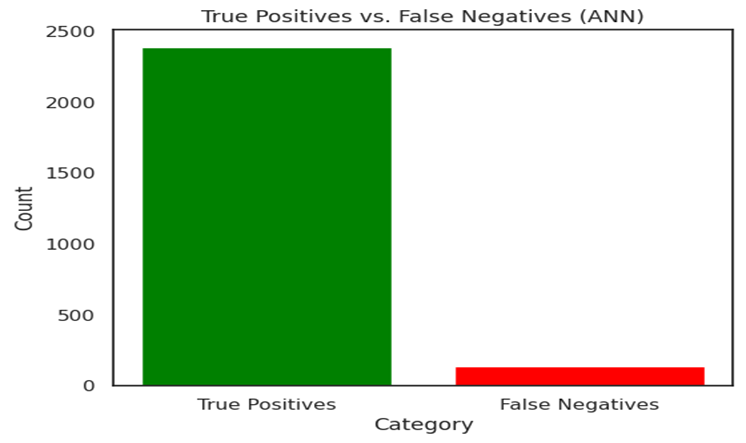
\includegraphics[width=0.59\textwidth]{8.png}}
    \subfigure{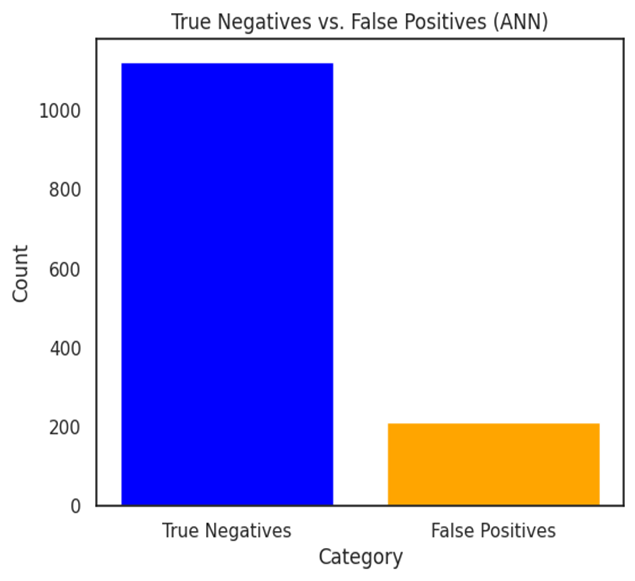
\includegraphics[width=0.49\textwidth]{9.png}}
    \caption{\small{TP vs FN and TN vs FP for the ANN model}}
    \label{fig:abc}
\end{figure}
\begin{figure}[htbp]
\hspace{-1.5cm}
    \subfigure{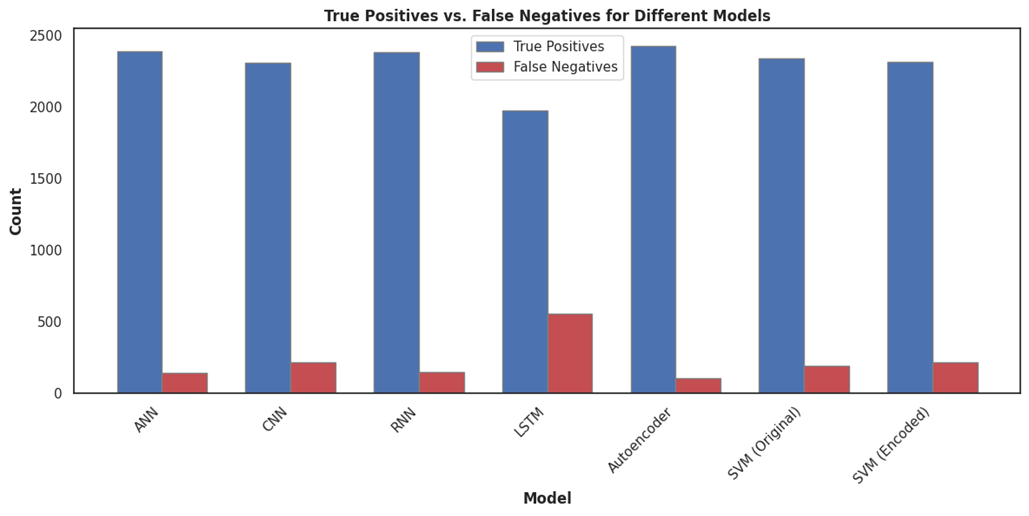
\includegraphics[width=0.59\textwidth]{10.png}}
    \subfigure{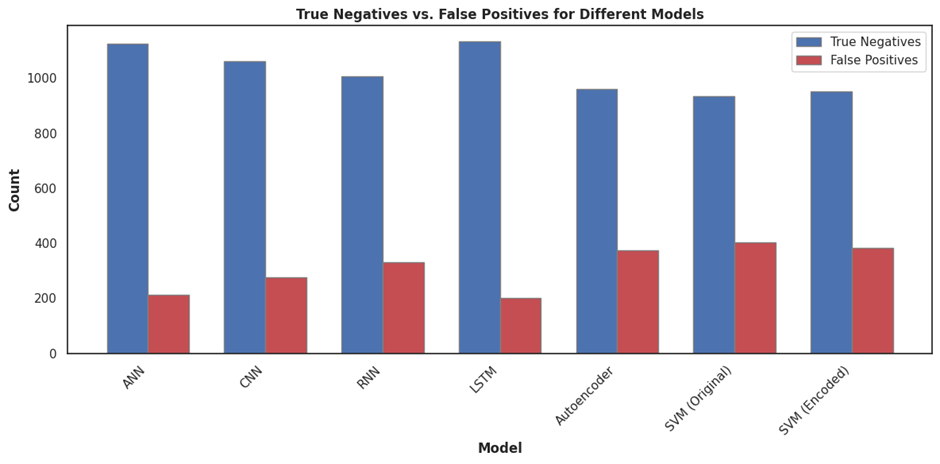
\includegraphics[width=0.59\textwidth]{11.png}}
    \caption{\small{TP vs FN and TN vs FP for the other models}}
    \label{fig:abc}
\end{figure}


To conclude, the study demonstrated that deep learning techniques especially, an improved variation of artificial neural networks employing algorithms like SCG ,LM and BR, can be used to advance cloud security  and adjustments of hyperparameters and datasets integration (UNSW-NB15 and CICIDS 2017), the model reached an impressive threat detection accuracy, indicating its suitability for real-time threat detection and embedding into multilayer cloud security systems[6].


\begin{table}[htbp]
\caption{Accuraries of both datasets}
\centering
\begin{tabular}{|c|c|c|}
        \hline
        SNo & Dataset & Model Accuracy \\ \hline
        1 & UNSW-NB15 & 90.12 \\ \hline
        2 & CICIDS-2017 & 80.18 \\ \hline
\end{tabular}
\label{tab 2}
\end{table}
The table-4 shows how accurate the threat detection model is in regards to two datasets, UNSW-NB15 and CICIDS 2017, in the context of cloud computing. In this model, the highest accuracy was reported for the UNSW-NB15 dataset, which reached 90.12 percent. It was 80.18 percent for the accuracy for the CICIDS 2017 data [13]. Hence, the model is more effective in spotting security threats in UNSW-NB15 datasets rather than others, although they can be detected on other datasets too. The results bring to focus how neural networks and their variants have contributed towards the enhancement of cloud systems in terms of timely threat detection [14].

\section{Result}

This paper developed an effective intelligence-based model to enhance cloud security through the detection of cyber attacks. By using advanced training techniques such as Levenberg-Marquardt, Scaled Conjugate Gradient, and Bayesian Regularization, the study was able to achieve improvements in detection of accuracy when validated on UNSW-NB15 and CICIDS 2017 datasets.These algorithms can be used to enhance the model and increase the accuracy of the model.The paper stressed the importance of algorithm selection and hyperparameter tuning while aiming at enhancing the performance of the ANN architecture. In addition, further comparative analysis with other models has confirmed the ability of the ANN to perform real-time threat detection in clouds. This study shows that the construction of ANNs in the current environment, with all tools and equipment for cloud security, will be able to cope effectively with the new type of cyber threats. It constitutes a flexible and effective partial solution in fighting future advanced threats targeting largely adopted cloud services.



%
% ---- Bibliography ----
%
% BibTeX users should specify bibliography style 'splncs04'.
% References will then be sorted and formatted in the correct style.
%
% \bibliographystyle{splncs04}
% \bibliography{mybibliography}
%
\begin{thebibliography}{8}
\bibitem{RefJ}
Kale, V. (2014). Guide to cloud computing for business and technology managers: from distributed computing to cloudware applications. CRC Press.
\bibitem{RefB}
Hasimi, L., Zavantis, D., Shakshuki, E., & Yasar, A. (2024). Cloud computing security and deep learning: An ANN approach. Procedia Computer Science, 231, 40-47.

\bibitem{RefB}
Gupta, A., & Kalra, M. (2020, November). Intrusion Detection and Prevention system using Cuckoo search algorithm with ANN in Cloud Computing. In 2020 Sixth international conference on parallel, distributed and grid computing (PDGC) (pp. 66-72). IEEE.
\bibitem{RefB}
(https://www.Kaggle.Com/datasets/chethuhn/community-intrusion-dataset),(https://www.Kaggle.Com/datasets/dhoogla/unswnb15),
 
 (https://www.kaggle.com /datasets/ hassan06/nslkdd).
\bibitem{RefB}
Etaiwi, W., & Naymat, G. (2017). The impact of applying different preprocessing steps on review spam detection. Procedia computer science, 113, 273-279.
\bibitem{RefB}
Subramanian, E. K., & Tamilselvan, L. (2019). A focus on future cloud: machine learning-based cloud security. Service Oriented Computing and Applications, 13(3), 237-249.
\bibitem{RefB}
Zarai, R. (2020). Recurrent Neural Networks & Deep Neural Networks Based on Intrusion Detection System. Open Access Library Journal, 7(03), 1.
\bibitem{RefB}
Nassif, A. B., Talib, M. A., Nasir, Q., Albadani, H., & Dakalbab, F. M. (2021). Machine learning for cloud security: a systematic review. IEEE Access, 9, 20717-20735.
\bibitem{RefB}
Rauber, P. E., Fadel, S. G., Falcao, A. X., & Telea, A. C. (2016). Visualizing the hidden activity of artificial neural networks. IEEE transactions on visualization and computer graphics, 23(1), 101-110..
\bibitem{RefB}
Srikanth, N., & Jacob, T. P. (2021, November). An Real Time Cloud Security System and Issues comparison using Machine and Deep Learning. In 2021 Fifth International Conference on I-SMAC (IoT in Social, Mobile, Analytics and Cloud)(I-SMAC) (pp. 523-529). IEEE.
\bibitem{RefB}
Humphrey, G. B., Maier, H. R., Wu, W., Mount, N. J., Dandy, G. C., Abrahart, R. J., & Dawson, C. W. (2017). Improved validation framework and R-package for artificial neural network models. Environmental Modelling & Software, 92, 82-106.
\bibitem{ref12}
Fan, C., Chen, M., Wang, X., Wang, J., & Huang, B. (2021). A review on data preprocessing techniques toward efficient and reliable knowledge discovery from building operational data. Frontiers in Energy Research, 9, 652801.
 \bibitem{ref13}
Ferrag, M. A., Friha, O., Hamouda, D., Maglaras, L., & Janicke, H. (2022). Edge-IIoTset: A new comprehensive realistic cyber security dataset of IoT and IIoT applications for centralized and federated learning. IEEE Access, 10, 40281-40306.
 \bibitem{ref14}
Sana, M. U., Li, Z., Javaid, F., Liaqat, H. B., & Ali, M. U. (2021). Enhanced security in cloud computing using neural network and encryption. IEEE Access, 9, 145785-145799.
\bibitem{ref15}
 Oyinloye, T. S., Arowolo, M. O., & Prasad, R. (2024). Enhancing Cyber Threat Detection with an Improved Artificial Neural Network Model. Data Science and Management.

\end{thebibliography}
\end{document}
